\documentclass[a4paper]{article}
\usepackage[a4paper,margin=0mm]{geometry}
\usepackage{fontspec}
\usepackage{unicode-math}
\usepackage{tikz}
\usepackage[table]{xcolor}
\usepackage[absolute]{textpos}
\usepackage{enumitem}
\usepackage{array}
\usepackage{multirow}

\setmainfont{Libertinus Serif}
\setsansfont{Libertinus Sans}
\setmathfont{Libertinus Math}
\newfontfamily\trackedsans{Libertinus Sans}[LetterSpace=8.0]

\definecolor{accent}{HTML}{602785}
\definecolor{badge}{HTML}{B8A0C8}
\definecolor{ink}{HTML}{2A2E30}

\setlength{\TPHorizModule}{1mm}
\setlength{\TPVertModule}{1mm}
\setlength{\parindent}{0pt}
\pagestyle{empty}

\newcommand{\LCOL}{16mm}
\newcommand{\RCOL}{111mm}
\newcommand{\COLW}{83mm}

\newcommand{\topicheader}[2]{%
\begin{textblock*}{194mm}(16mm,10mm)
\begin{tikzpicture}
\node[fill=accent,text=white,font=\sffamily\bfseries\fontsize{13}{13}\selectfont,
      minimum width=9mm,minimum height=9mm,inner sep=0pt] at (4.5mm,-4.5mm) {#1};
\node[font=\sffamily\bfseries\fontsize{15}{16}\selectfont,text=ink,anchor=west] at (12mm,-4.5mm) {#2};
\end{tikzpicture}
\end{textblock*}
\begin{textblock*}{194mm}(16mm,22.5mm)

\begin{tikzpicture}
\fill[accent] (0,0) rectangle (194mm,0.5mm);
\end{tikzpicture}
\end{textblock*}
}

\newcommand{\pagefooter}[1]{%
\begin{textblock*}{194mm}(8mm,286.41mm)
  
\begin{tikzpicture}
    \fill[accent] (0,0) rectangle (194mm,0.6mm);
  \end{tikzpicture}
\end{textblock*}
\begin{textblock*}{63.59mm}(8mm,288.27mm)
  {\sffamily\bfseries\color{accent}\fontsize{13}{16}\selectfont SAT 1200+}
\end{textblock*}
\begin{textblock*}{10mm}(188mm,288.27mm)
  \centering{\sffamily\color{accent}\fontsize{14}{16}\selectfont #1}
\end{textblock*}
}

\newcommand{\colrule}[2]{%
\begin{textblock*}{1mm}(105mm,#1mm)
\begin{tikzpicture}
\draw[black!65,line width=0.5pt] (0,0) -- (0,#2mm);
\end{tikzpicture}
\end{textblock*}
}

\newcommand{\setkicker}[2]{%
{\sffamily\bfseries\fontsize{12}{14}\selectfont #1.}\ {\itshape\fontsize{11}{14}\selectfont\color{black!75} #2}\par\vspace{2mm}%
}

\setlength{\fboxsep}{1.4pt}
\setlength{\fboxrule}{0.5pt}
\newcommand{\pnum}[1]{\fcolorbox{ink}{white}{\sffamily\bfseries\fontsize{8}{8}\selectfont #1}~}

\newcommand{\qrbox}[1]{%
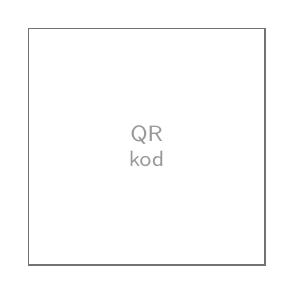
\begin{tikzpicture}
\draw[black!55,line width=0.6pt] (0,0) rectangle (30mm,30mm);
\node[black!40,font=\sffamily\fontsize{8}{9}\selectfont,align=center] at (15mm,15mm) {QR\\kod};
\end{tikzpicture}\\[1.5mm]
{\sffamily\fontsize{9}{11}\selectfont\color{black!70} #1}%
}

\arrayrulecolor{accent}
\setlength{\arrayrulewidth}{0.7pt}
\renewcommand{\arraystretch}{1.35}
\newcommand{\anstitle}[1]{{\sffamily\bfseries\color{accent}\fontsize{11}{13}\selectfont #1}\\[1.3mm]}

\begin{document}

% ================= PAGE 1: Set 1 | Set 2 =================
\topicheader{9}{Ko'phadlar ustida amallar}
\pagefooter{1}
\colrule{32}{238}
\mbox{}%

\begin{textblock*}{\COLW}(\LCOL,32mm)
{\fontsize{12}{15}\selectfont
\setkicker{1-to'plam}{Qo'shish/ayirish -- ayirish ishorasi qopqoniga e'tibor bering.}

\noindent\pnum{1} $(3x^2+2x-5)+(x^2-4x+7)=$\\[22mm]
\noindent\pnum{2} $(5x^3-2x+1)-(2x^3+3x-4)=$\\[22mm]
\noindent\pnum{3} $(-2x^2+6x-3)+(4x^2-6x+8)=$\\[22mm]
\noindent\pnum{4} $(6x^2-3x)-(2x^2-3x+5)=$\\[22mm]
\noindent\pnum{5} $(x^3+2x^2-x)+(-x^3+5x-3)=$\\[22mm]
\noindent\pnum{6} $(4x^2+7)-(x^2-2x+7)=$
}
\end{textblock*}

\begin{textblock*}{\COLW}(\RCOL,32mm)
{\fontsize{12}{15}\selectfont
\setkicker{2-to'plam}{Binomlarni ko'paytirish (FOIL usuli).}

\noindent\pnum{1} $(x+3)(x+5)=$\\[22mm]
\noindent\pnum{2} $(x-2)(x+7)=$\\[22mm]
\noindent\pnum{3} $(2x+1)(x-4)=$\\[22mm]
\noindent\pnum{4} $(x-6)(x-6)=$\\[22mm]
\noindent\pnum{5} $(3x+2)(3x-2)=$\\[22mm]
\noindent\pnum{6} $(x+4)(2x^2-x+3)=$
}
\end{textblock*}

\clearpage

% ================= PAGE 2: Set 3 | Set 4 =================
\topicheader{9}{Ko'phadlar ustida amallar}
\pagefooter{2}
\colrule{32}{238}
\mbox{}%

\begin{textblock*}{\COLW}(\LCOL,32mm)
{\fontsize{12}{15}\selectfont
\setkicker{3-to'plam}{Qiyinroq ko'paytirish -- kvadratlar, binom$\times$trinom, uch ko'paytuvchi.}

\noindent\pnum{1} $(x+2)^2=$\\[22mm]
\noindent\pnum{2} $(2x-1)^2=$\\[22mm]
\noindent\pnum{3} $(x^2+3x-2)(x+4)=$\\[22mm]
\noindent\pnum{4} $(x-1)(x^2+x+1)=$\\[22mm]
\noindent\pnum{5} $(3x+1)(x^2-2x+5)=$\\[22mm]
\noindent\pnum{6} $(x+2)(x-2)(x+1)=$
}
\end{textblock*}

\begin{textblock*}{\COLW}(\RCOL,32mm)
{\fontsize{12}{15}\selectfont
\setkicker{4-to'plam}{Bo'lish.}

\noindent\pnum{1} $(6x^3-9x^2+3x)\div3x=$\\[22mm]
\noindent\pnum{2} $(8x^2+12x)\div4x=$\\[22mm]
\noindent\pnum{3} $(10x^4-5x^3+15x^2)\div5x^2=$\\[22mm]
\noindent\pnum{4} $(x^2+5x+6)\div(x+2)=$\\[22mm]
\noindent\pnum{5} $(x^2-9)\div(x-3)=$\\[22mm]
\noindent\pnum{6} $(2x^2+7x+3)\div(2x+1)=$
}
\end{textblock*}

\clearpage

% ================= PAGE 3: Set 5 | Set 6 (spot the error) =================
\topicheader{9}{Ko'phadlar ustida amallar}
\pagefooter{3}
\colrule{32}{238}
\mbox{}%

\begin{textblock*}{\COLW}(\LCOL,32mm)
{\fontsize{12}{15}\selectfont
\setkicker{5-to'plam}{Aralash -- bir masalada bir nechta amal, haqiqiy test zichligi.}

\noindent\pnum{1} $(x+3)(x-2)-(x^2-5)=$\\[22mm]
\noindent\pnum{2} $(2x-1)(x+4)+(x^2+3x)=$\\[22mm]
\noindent\pnum{3} $(x+5)^2-(x^2+10)=$\\[22mm]
\noindent\pnum{4} $(3x^2-2x+1)-(x+2)(x-1)=$\\[22mm]
\noindent\pnum{5} $2(x+1)(x-1)+(x^2-3)=$\\[22mm]
\noindent\pnum{6} $(x-4)^2+(8x-10)=$
}
\end{textblock*}

\begin{textblock*}{\COLW}(\RCOL,32mm)
{\fontsize{11}{14}\selectfont
\setkicker{6-to'plam}{Xatoni toping -- buzilgan qadamni ayting, to'g'ri javobni bering.}

\noindent\pnum{1} $(x^2+3x)-(x^2-2x+5)$ ifodasida ko'rsatilgan yechimda xato bor:\\[1mm]
\hspace*{7mm}\textit{``$x^2+3x-x^2-2x+5=x+5$.''}\\[2mm]
\hspace*{7mm}Xato va to'g'ri javob: \makebox[52mm]{\dotfill}\\[6mm]

\noindent\pnum{2} $(x+3)(x-4)$ ifodasida ko'rsatilgan yechimda xato bor:\\[1mm]
\hspace*{7mm}\textit{``$x\times x+3\times(-4)=x^2-12$.''}\\[2mm]
\hspace*{7mm}Xato va to'g'ri javob: \makebox[52mm]{\dotfill}\\[6mm]

\noindent\pnum{3} $3x\times(-5x)$ ifodasida ko'rsatilgan yechimda xato bor:\\[1mm]
\hspace*{7mm}\textit{``$=+15x^2$.''}\\[2mm]
\hspace*{7mm}Xato va to'g'ri javob: \makebox[52mm]{\dotfill}\\[6mm]

\noindent\pnum{4} $x^2+x^2$ ifodasida ko'rsatilgan yechimda xato bor:\\[1mm]
\hspace*{7mm}\textit{``$=x^4$.''}\\[2mm]
\hspace*{7mm}Xato va to'g'ri javob: \makebox[52mm]{\dotfill}\\[6mm]

\noindent\pnum{5} $(8x^2+4x)\div4x$ ifodasida ko'rsatilgan yechimda xato bor:\\[1mm]
\hspace*{7mm}\textit{``$8x^2\div4x=2x$, demak javob $2x+4x=6x$.''}\\[2mm]
\hspace*{7mm}Xato va to'g'ri javob: \makebox[52mm]{\dotfill}
}
\end{textblock*}

\clearpage

% ================= PAGE 4: Set 7 (bonus) -- own page =================
\topicheader{9}{Ko'phadlar ustida amallar}
\pagefooter{4}
\colrule{32}{238}
\mbox{}%

\begin{textblock*}{\COLW}(\LCOL,32mm)
{\fontsize{12}{15}\selectfont
\setkicker{7-to'plam}{Bonus / qiyin -- har biriga taxminan 90 soniya.}

\noindent\pnum{1} $(x+1)(x+2)(x+3)=$\\[26mm]
\noindent\pnum{2} $(x^2+2x+1)\div(x+1)=$\\[26mm]
\noindent\pnum{3} $(3x-2)(2x+5)-(x-1)(x+6)=$\\[26mm]
\noindent\pnum{4} $(x+4)^2-(x-4)^2=$\\[26mm]
\noindent\pnum{5} $(2x^2-3x+1)\div(2x-1)=$
}
\end{textblock*}

\clearpage

% ================= PAGE 5: Javoblar -- full-page answer table =================
\topicheader{9}{Ko'phadlar ustida amallar}
\pagefooter{5}
\mbox{}%

\begin{textblock*}{194mm}(16mm,30mm)
{\bfseries\itshape\color{accent}\fontsize{19}{21}\selectfont\centering Javoblar\par}
\end{textblock*}

\begin{textblock*}{194mm}(16mm,44mm)
{\fontsize{9.3}{11.5}\selectfont
\centering
\renewcommand{\arraystretch}{1.3}
\begin{tabular}{|>{\centering\arraybackslash}p{20mm}|>{\centering\arraybackslash}p{7mm}|>{\centering\arraybackslash}p{36mm}|>{\centering\arraybackslash}p{7mm}|>{\centering\arraybackslash}p{36mm}|}
\hline
\rowcolor{badge!55}\textbf{To'plam} & \textbf{\#} & \textbf{Javob} & \textbf{\#} & \textbf{Javob}\\
\hline
\multirow{3}{20mm}{\centering 1-to'plam} & 1 & $4x^2-2x+2$ & 2 & $3x^3-5x+5$\\\cline{2-5}
 & 3 & $2x^2+5$ & 4 & $4x^2-5$\\\cline{2-5}
 & 5 & $2x^2+4x-3$ & 6 & $3x^2+2x$\\\hline
\multirow{3}{20mm}{\centering 2-to'plam} & 1 & $x^2+8x+15$ & 2 & $x^2+5x-14$\\\cline{2-5}
 & 3 & $2x^2-7x-4$ & 4 & $x^2-12x+36$\\\cline{2-5}
 & 5 & $9x^2-4$ & 6 & $2x^3+7x^2-x+12$\\\hline
\multirow{3}{20mm}{\centering 3-to'plam} & 1 & $x^2+4x+4$ & 2 & $4x^2-4x+1$\\\cline{2-5}
 & 3 & $x^3+7x^2+10x-8$ & 4 & $x^3-1$\\\cline{2-5}
 & 5 & $3x^3-5x^2+13x+5$ & 6 & $x^3+x^2-4x-4$\\\hline
\multirow{3}{20mm}{\centering 4-to'plam} & 1 & $2x^2-3x+1$ & 2 & $2x+3$\\\cline{2-5}
 & 3 & $2x^2-x+3$ & 4 & $x+3$\\\cline{2-5}
 & 5 & $x+3$ & 6 & $x+3$\\\hline
\multirow{3}{20mm}{\centering 5-to'plam} & 1 & $x-1$ & 2 & $3x^2+10x-4$\\\cline{2-5}
 & 3 & $10x+15$ & 4 & $2x^2-3x+3$\\\cline{2-5}
 & 5 & $3x^2-5$ & 6 & $x^2+6$\\\hline
\multirow{3}{20mm}{\centering 7-to'plam} & 1 & $x^3+6x^2+11x+6$ & 2 & $x+1$\\\cline{2-5}
 & 3 & $5x^2+6x-4$ & 4 & $16x$\\\cline{2-5}
 & 5 & $x-1$ & -- & --\\\hline
\multirow{5}{20mm}{\centering 6-to'plam} & \multicolumn{4}{p{86mm}|}{1.\ Faqat birinchi had ishorasi o'zgartirildi, ikkinchi qavs ichidagi barcha hadlar ishorasini almashtirish kerak. To'g'ri: $5x-5$.}\\\cline{2-5}
 & \multicolumn{4}{p{86mm}|}{2.\ Faqat Birinchi va Oxirgi hadlar ko'paytirildi (FOIL to'liq emas) -- Tashqi va Ichki hadlar tushib qolgan. To'g'ri: $x^2-x-12$.}\\\cline{2-5}
 & \multicolumn{4}{p{86mm}|}{3.\ Manfiy$\times$manfiy musbat berishi kerak, bu yerda musbat$\times$manfiy bo'lgani uchun natija manfiy. To'g'ri: $-15x^2$.}\\\cline{2-5}
 & \multicolumn{4}{p{86mm}|}{4.\ Darajalar ko'paytirishdagidek qo'shildi; bu o'xshash hadlarni qo'shish, daraja o'zgarmaydi. To'g'ri: $2x^2$.}\\\cline{2-5}
 & \multicolumn{4}{p{86mm}|}{5.\ Faqat birinchi had $4x$ ga bo'lindi, ikkinchi had ham bo'linishi kerak. To'g'ri: $2x+1$.}\\\hline
\end{tabular}
}
\end{textblock*}

\begin{textblock*}{194mm}(16mm,248mm)
\centering
{\sffamily\fontsize{9.5}{11.5}\selectfont\color{black!70} Video yechimlar va qo'shimcha testlar uchun quyidagi QR kodlarni skanerlang:}\\[4mm]
\begin{minipage}[t]{32mm}\centering\qrbox{YouTube}\end{minipage}%
\hspace{16mm}%
\begin{minipage}[t]{32mm}\centering\qrbox{Telegram}\end{minipage}
\end{textblock*}

\end{document}
